\documentclass{beamer}
%\usepackage[bars]{beamerthemetree} % Beamer主题样式v 2.2
\usepackage{ctex}
\usepackage{amsmath}
\usepackage{bm}
\usepackage{cite}
\usepackage{color}
\usepackage{xcolor}
\usepackage{graphicx}
\usepackage{diagbox}

%\setbeamertemplate{bibliography item}[text]
\setbeamertemplate{bibliography item}{\insertbiblabel}
\setbeamertemplate{bibliography entry title}{}
\setbeamertemplate{bibliography entry location}{}
\setbeamertemplate{bibliography entry note}{}

\setbeamertemplate{caption}[numbered]


\usetheme{Warsaw} % Beamer主题样式v 3.0
% \usecolortheme{lily} % Beamer颜色主题样式
\usefonttheme{serif}

\graphicspath{{fig/}}

\newcommand{\upcite}[1]{\textsuperscript{\cite{#1}}}  %自定义命令\upcite, 使参考文献引用以上标出现
\newcommand{\M}[1]{\mathrm{#1}}

\newcommand{\R}[1]{\textcolor{red}{#1}}

\newcommand{\PP}[2]{\frac{\partial #1}{\partial #2}}
\newcommand{\PPP}[2]{\frac{\partial^{2} #1}{{\partial #2}^{2}}}

\newcommand{\DD}[2]{\frac{\mathrm{d} #1}{\mathrm{d} #2}}
\newcommand{\DDD}[2]{\frac{\mathrm{d}^{2} #1}{{\mathrm{d} #2}^{2}}}

    
\logo{
\includegraphics[height=0.1\textwidth]{bnu-fig-logo.pdf}}
\title{等温捷径与绝热捷径构成的类卡诺热机的效率与功率}
\author{龚政楠}
\institute{北京师范大学}
\begin{document}

\begin{frame} % Cover slide
\titlepage
\end{frame}

\begin{frame}           %生成目录页,目录太长时加选项[shrink]
    %	\setcounter{page}{0}	%setcounter似乎对beamer无效
        \addtocounter{framenumber}{-2}%---------位置放在beginframe之后,不然无效
        \frametitle{目录}
        \tableofcontents 
\end{frame}

%也可以用 \frame{\titlepage}}代替 (在Beamer v 2.2 宏包中)
\section{引言:热机的功率与效率问题}

% \begin{frame}{引言:热机的功率与效率问题}
% \end{frame}

\begin{frame}{引言:热机的功率与效率问题}
    \begin{itemize}
        \item<2-> 1824,卡诺指出\upcite{2005}:工作在相同高温热源和相同低温热源的所有热机中,以可逆热机的效率最高,为$\eta _{\mathrm{c}}=1-\frac{T_\mathrm{c}}{T_\mathrm{h}}$ 
        \item<3-> 1975年,Curzon和Ahlborn研究了内可逆热机\upcite{Curzon1975},得到了该热机在最大功率下的效率为$\eta _{\mathrm{CA}}=1-\sqrt{1-\eta _{\mathrm{c}}}$
        \item<4-> 2008年,T. Schmiedl 和 U. Seifert提出了布朗随机热机模型\upcite{Schmiedl2008},最大功率下的效率为$\frac{ \eta_{\mathrm{c}}}{2-\frac{1}{2}\eta_{\mathrm{c}}}$
        \item<5-> 同年,涂展春推导出费曼棘轮热机\upcite{Tu2008}在最大功率下的效率$\frac{\eta _{\mathrm{c}}^{2}}{\eta _{\mathrm{c}}-\left( 1-\eta _{\mathrm{c}} \right) \ln \left( 1-\eta _{\mathrm{c}} \right)}$. \upcite{Tu2020}
        \item<6-> 2013年,涂展春在Schmiedl和Seifert工作\upcite{Schmiedl2008}的基础上,考虑了他们在过阻尼情况下忽略的惯性的影响,构建了一种类卡洛热机\upcite{Tu2013}. 发现这种随机热机在最大功率下的效率等于$\eta _{\mathrm{CA}}$
    \end{itemize}    
\end{frame}


% \subsection{有限时间热机模型}
% \begin{frame}{CA内可逆热机模型}
% \begin{columns}
%     \begin{column}{.62\textwidth}
%         \begin{exampleblock}{Curzon和Ahlborn的假设}
%             \begin{itemize}
%                 \item<2-> 内可逆假设
%                 \item<3-> 绝热过程熵产生为零
%                 \item<4-> 绝热过程与等温过程所用的时间成正比,即循环总时间为$t_0 = a (t_{\mathrm{h}}+t_{\mathrm{c}})$
%                 \item<5-> 线性热传输假设,即
%                 \begin{equation}
%                     \begin{split}
%                         Q_{\mathrm{h}}&=\kappa_{\mathrm{h}}\left(T_{\mathrm{h}}-T_{\mathrm{eh}}\right) t_{\mathrm{h}}\\
%                         Q_{\mathrm{c}}&=\kappa_{\mathrm{c}}\left(T_{\mathrm{ec}}-T_{\mathrm{c}}\right) t_{\mathrm{c}}
%                     \end{split} 
%                     \label{eq1}
%                 \end{equation}
%             \end{itemize}   
%         \end{exampleblock}
%     \end{column}

%     \begin{column}{.38\textwidth}
%         \begin{figure}[!htbp]
%             \begin{center}
%                 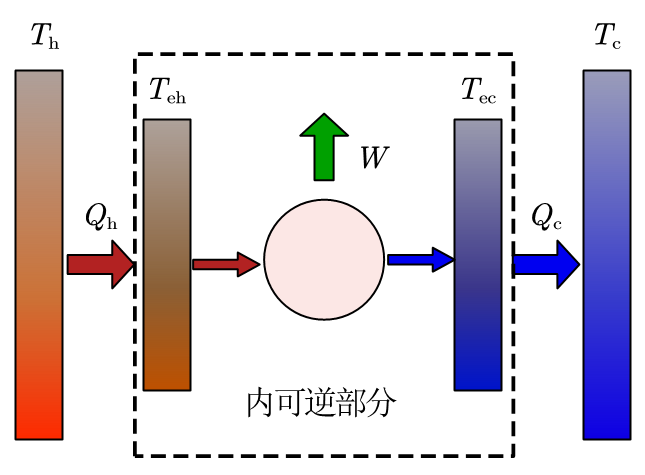
\includegraphics[width=\textwidth]{p1.png}
%             \end{center}
%             \caption{CA内可逆热机}
%             \label{f1}
%         \end{figure}
%     \end{column}
% \end{columns}
% \end{frame}

% \begin{frame}{CA内可逆热机模型}
%     \begin{columns}
%         \begin{column}{.62\textwidth}
%             \begin{block}{CA热机的功率}
%                 \pause
%                 输出功率
%                 \begin{equation}
%                     P\left(T_{\mathrm{eh}}, T_{\mathrm{ec}}\right)=\frac{T_{\mathrm{eh}}-T_{\mathrm{ec}}}{\frac{T_{\mathrm{eh}}}{a \kappa_{h}\left(T_{h}-T_{\mathrm{eh}}\right)}+\frac{T_{\mathrm{ec}}}{a \kappa_{c}\left(T_{\mathrm{ec}}-T_{c}\right)}}
%                     \label{eq2}
%                 \end{equation}
%                 \pause 针对$T_{\mathrm{eh}}, T_{\mathrm{ec}}$使功率取最大值
%                 \begin{equation}
%                     \begin{split}
%                         T_{\mathrm{eh}}^{*}&=\frac{\sqrt{\kappa_{h} T_{h}}+\sqrt{\kappa_{c} T_{c}}}{\sqrt{\kappa_{h}}+\sqrt{K_{c}}} \sqrt{T_{h}}\\
%                         T_{\mathrm{ec}}^{*}&=\frac{\sqrt{\kappa_{h} T_{h}}+\sqrt{\kappa_{c} T_{c}}}{\sqrt{K_{h}}+\sqrt{\kappa_{c}}} \sqrt{T_{c}}
%                     \end{split}
%                     \label{eq3}
%                 \end{equation}
%             \end{block}
%         \end{column}
    
%         \begin{column}{.38\textwidth}
%             \onslide
%             \begin{figure}
%                 \begin{center}
%                     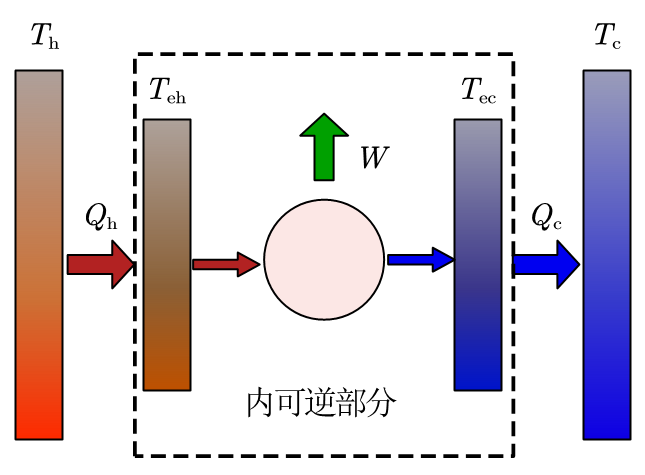
\includegraphics[width=\textwidth]{p1.png}
%                 \end{center}
%                 \setcounter{figure}{0}
%                 \caption{CA内可逆热机}
%             \end{figure}
%         \end{column}
%     \end{columns}
% \end{frame}

% \begin{frame}{CA内可逆热机模型}
%     \begin{alertblock}{CA热机在最大功率下的效率}
%         根据$\eta=1-T_{\mathrm{ec}} / T_{\mathrm{eh}}$就可以得到
%         \begin{equation}
%             \eta _{\mathrm{CA}}=1-\sqrt{1-\eta _{\mathrm{C}}}
%             \label{eq4}
%         \end{equation}
%     \end{alertblock}
% \end{frame}

% \begin{frame}{TU布朗随机热机模型}
%     \begin{columns}
%         \begin{column}{.62\textwidth}
%             \begin{exampleblock}{TU布朗随机热机的假设}
%                 \begin{itemize}
%                     \item<2->  两个绝热过程是在瞬间完成的,$t_0 = (t_{\mathrm{h}}+t_{\mathrm{c}})$
%                     \item<3->  两个绝热过程中不可逆熵产生为零
%                     \item<4->  过阻尼假设,不考虑惯性的影响
%                 \end{itemize}         
%             \end{exampleblock}
%         \end{column}
    
%         \begin{column}{.38\textwidth}
%             \onslide
%             \begin{figure}
%                 \begin{center}
%                     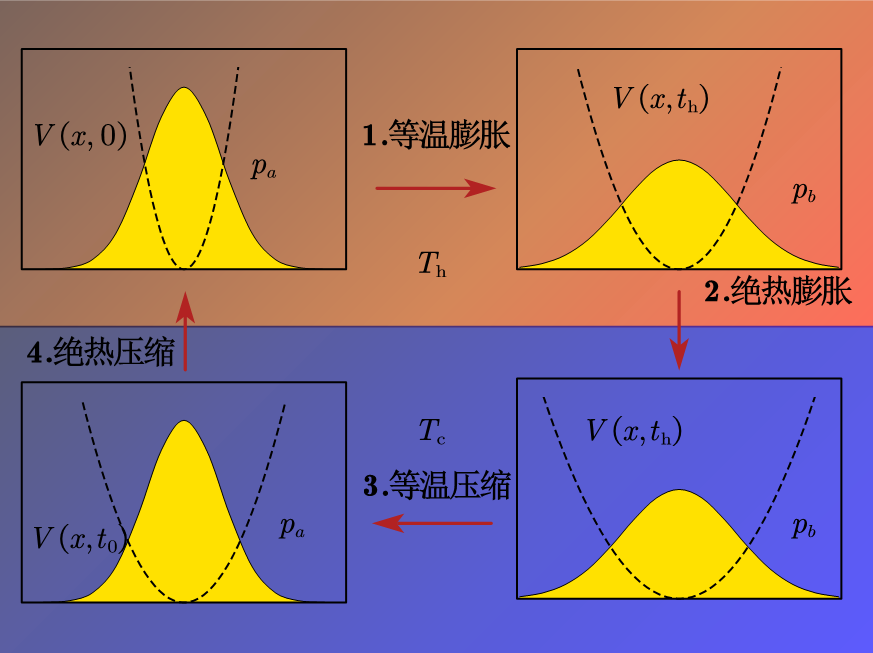
\includegraphics[width=\textwidth]{p2.png}
%                 \end{center}
%                 \caption{TU布朗随机热机模型}
%                 \label{f2}
%             \end{figure}
%         \end{column}
%     \end{columns}
% \end{frame}

% \begin{frame}{TU布朗随机热机的功率}
%     \begin{columns}
%         \begin{column}{.62\textwidth}
%             \begin{block}{TU布朗随机热机}
%                 \pause
%                 平均功输出  
%                     \begin{equation}
%                         \begin{split}
%                             -W=\left(T_{\mathrm{h}}-T_{\mathrm{c}}\right) \Delta S-\left({1}/{t_{\mathrm{h}}}+{1}/{t_{\mathrm{c}}}\right) A_{\mathrm{irr}}
%                         \end{split} 
%                         \label{eq5}
%                     \end{equation}
%                     \pause
%                     吸收热
%                     \begin{equation}
%                         \begin{split}
%                             Q =T_{\mathrm{h}} \Delta S-{A_{\mathrm{irr}}}/{t_{\mathrm{h}}}
%                         \end{split}
%                         \label{eq6}
%                     \end{equation}
%                     \pause
%                     功率
%                     \begin{equation}
%                         \begin{split}
%                             P=\frac{\left(T_{\mathrm{h}}-T_{\mathrm{c}}\right) \Delta S-\left({1}/{t_{\mathrm{h}}}+{1}/{t_{\mathrm{c}}}\right) A_{\mathrm{irr}}}{t_{\mathrm{h}} + t_{\mathrm{c}}}
%                         \end{split}
%                         \label{eq7}
%                     \end{equation}       
%             \end{block}
%         \end{column}
    
%         \begin{column}{.38\textwidth}
%             \onslide
%             \begin{figure}
%                 \begin{center}
%                     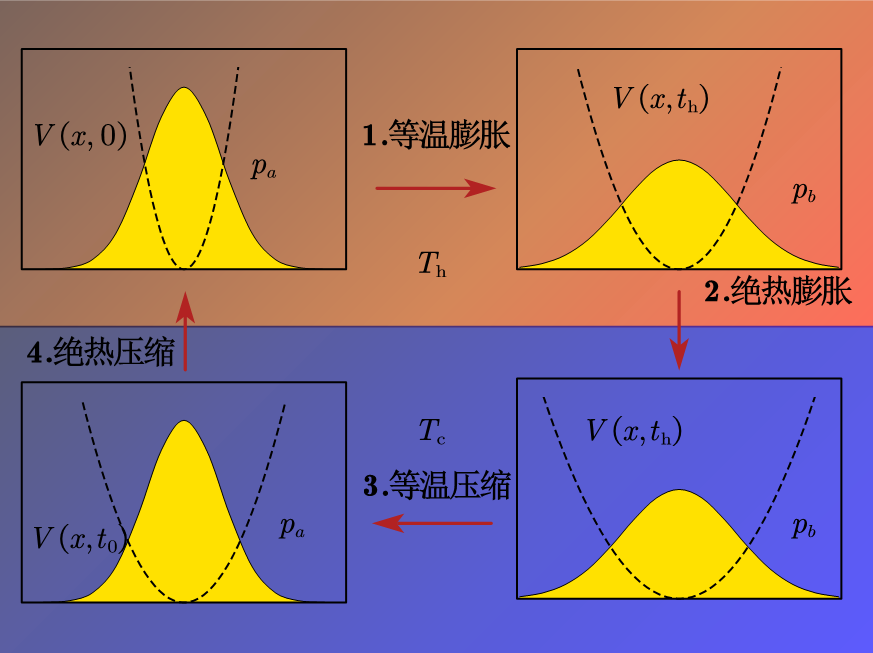
\includegraphics[width=\textwidth]{p2.png}
%                 \end{center}
%                 \setcounter{figure}{1}
%                 \caption{TU布朗随机热机模型}
%             \end{figure}
%         \end{column}
%     \end{columns}
% \end{frame}

% \begin{frame}{TU布朗随机热机}
% \begin{alertblock}{TU布朗随机热机的效率}
% 通过优化$t_1,\ t_2$不难得到,最大功率时的效率为
% \begin{equation}
%     \eta^{*}=\frac{\eta_{\mathrm{C}}}{2-\eta_{\mathrm{C}} / 2}
%     \label{eq8}
% \end{equation}
% \end{alertblock}
% \end{frame}
\section{绝热捷径与等温捷径简介}
\subsection{绝热捷径}
\begin{frame}{绝热捷径}
为了在有限时间内实现平衡态的转化, Demirplak and Rice \upcite{Demirplak2003}和 Berry \upcite{Berry2009} 独立发展出了绝热捷径的策略。
\pause

对于依赖于时间缓变的$H_0(t)$,有绝热定理\upcite{Griffiths2018}
\begin{equation}
\begin{split}
    |\psi(t)\rangle=&|n(t)\rangle e^{i \theta_{n}(t)} e^{i \gamma_{n}(t)},\\
    \theta_{n}(t)=-\frac{1}{\hbar} \int_{0}^{t} E_{n}(t^{\prime}) \M{d} t^{\prime},& \quad \gamma_{n}(t)=i \int_{0}^{t}\langle n(t^{\prime}) | \partial_{t^{\prime}}n(t^{\prime})\rangle \M{d} t^{\prime}            
\end{split}        
    \label{eq9}
\end{equation}
\pause
若有$H(t)$使得绝热定理严格成立
\pause
\begin{equation}
\begin{split}
    H(t)&=H_{0}(t)+i \hbar \sum_{m}\left(\left|\partial_{t} m\right\rangle\left\langle m\left|-\left\langle m \mid \partial_{t} m\right\rangle\right| m\right\rangle\langle m|\right) \\
    &\equiv H_0 + H_1
\end{split}
    \label{eq10}
\end{equation}
\end{frame}

\begin{frame}{绝热捷径}
    在经典的情形下,对于随时间缓变的$H_0 (t)$,也可以引入辅助哈密顿量$H_1 (t)$,使得绝热不变量\upcite{LiuChuan2019}严格守恒
        \begin{equation}
            I(E, \boldsymbol{\lambda}) \equiv \int \mathrm{d} \bm{\eta} \theta\left[E-H_{0}(z ; \boldsymbol{\lambda})\right]
          \label{eq11}
        \end{equation}
        \pause
    \begin{alertblock}{谐振子势场中的辅助势}
        根据Jarzynski的计算\upcite{Jarzynski2013},对于依赖于时间的谐振子势
        \begin{equation}
            H_{0}(\bm{\eta} ; \lambda(t))=\frac{p^{2}}{2}+\frac{q^2}{2\lambda(t)^{2}}
            \label{eq12}
        \end{equation}
        \pause
        其相应的辅助势为
        \begin{equation}
            H_{1}(\bm{\eta} ; \lambda(t))=\frac{\dot{\lambda}}{2 \lambda} q p
            \label{eq13}
        \end{equation}
    \end{alertblock}
\end{frame}

% \begin{frame}{利用绝热捷径实现平衡态的转化}
% 考虑谐振子势式\eqref{eq12},施加辅助哈密顿量之后的新哈密顿量为
% \begin{equation}
%     H(t)=\frac{p^{2}}{2}+\frac{q^2}{2 \lambda(t)^{2}}+\frac{\dot{\lambda}}{2 \lambda(t)} q p,
%     \label{eq13.5}
% \end{equation}
% \pause
% 可以得到运动方程
% \begin{equation}
%     \left\{\begin{aligned}
%         &\dot{q}=\frac{\partial H}{\partial p}={p}+\frac{\lambda(t)}{2 \lambda(t)} q \\
%         &\dot{p}=-\frac{\partial H}{\partial q}=-2  \frac{q}{\lambda^{2}(t)}-\frac{\dot{\lambda}(t)}{2 \lambda(t)} p
%     \end{aligned}\right.
%     \label{eq14}
% \end{equation}
% \end{frame}

\begin{frame}{利用绝热捷径实现平衡态的转化}
\begin{alertblock}{平衡态的转化}
设初态为平衡态
\begin{equation}
    \rho_{i}=\frac{\beta_{i}}{2 \pi \lambda_{i}} \exp \left[-\beta_{i} H_0 \left(t_{i}\right)\right]
    \label{eq16}
\end{equation}
\pause
假设末态为等效温度为$\beta_{f}$的平衡态
\begin{equation}
    \rho_{f}=\frac{\beta_{f} }{2 \pi \lambda_{f}} \exp \left[-\beta_{f} H_0 \left(t_{f}\right)\right]
    \label{eq17}
\end{equation}
\pause
鉴于$\rho_{f}=\rho_{i}$,$\DD{H_0 (t)}{t}=-H_0 (t) \DD{\ln{\lambda(t)}}{t}$,得到\upcite{Tu2013}
\begin{equation}
    \frac{\beta_f}{\lambda_f} = \frac{\beta_i}{\lambda_i}
    \label{eq18}
\end{equation}
\end{alertblock}
\end{frame}
\subsection{等温捷径}
\begin{frame}{等温捷径}
为了实现等温平衡态之间的相互转化,类似于绝热捷径,李耿等人\upcite{Li2016}发展出了等温捷径的策略。

\pause

为系统施加一个额外的辅助势场,使得哈密顿量成为
\begin{equation}
    H(q, p, t)=H_{0}(q, p, \lambda(t))+U_{1}(q, p, t)
    \label{eq19}
\end{equation}
\pause
分布函数$\rho(q, p, t)$的演化由福克-普朗克方程决定
\begin{equation}
    \begin{split}
        \PP{\rho}{t} &+ \nabla \cdot \bm{J} = 0\\
        \bm{J} \equiv \rho \left( p + \PP{U}{p} \right) \hat{\mathbf{q}}&-\rho\left(\gamma p+\frac{\partial U}{\partial q}+ \PP{U}{p} + \frac{\gamma}{\rho \beta} \frac{\partial \rho}{\partial p}\right) \hat{\mathbf{p}}
    \end{split}
    \label{eq20}
\end{equation}
\end{frame}

\begin{frame}{等温捷径}
\begin{alertblock}{等温平衡态的转化}
系统在原哈密顿量$H_{0}(q, p, \lambda(t))$下的瞬时平衡态
\begin{equation}
    \begin{split}
        \rho(q, p, t) &= \mathrm{e}^{\beta\left[F(\lambda(t))-H_{0}(q, p, \lambda(t))\right]}
    \end{split}
    \label{eq21}
\end{equation}
\pause
要使系统始终保持瞬时平衡态,将上式\eqref{eq21}代入方程\eqref{eq20},得到\upcite{Li2016}
\begin{equation}
    \frac{\gamma}{\beta} \frac{\partial^{2} U_{1}}{\partial p^{2}}-\gamma p \frac{\partial U_{1}}{\partial p}+\frac{\partial U_{0}}{\partial q} \frac{\partial U_{1}}{\partial p}-p \frac{\partial U_{1}}{\partial q}=\left(\frac{d F}{d \lambda}-\frac{\partial U_{0}}{\partial \lambda}\right) \dot{\lambda}
    \label{eq22}
\end{equation}
\pause
利用上式\eqref{eq22},对依赖于时间的谐振子势$U_0 = q^{2} / 2 \lambda(t)^2$
\begin{equation}
    U_{1}(q, p, t)=-\frac{\dot{\lambda}(t)}{2 \gamma \lambda(t)}\left[(p-\gamma q)^{2}+ q^{2}/\lambda(t)^2\right]
    \label{eq2.62}
\end{equation}
\end{alertblock}
\end{frame} 

\section{类卡诺热机的功率与效率}
\subsection{布朗粒子能量学}
\begin{frame}{布朗粒子能量学}
\pause
哈密顿量为$H=\frac{p^{2}}{2}+U_0 (q,\lambda(t)) + U_1 (q,p,t)$,其全微分
\begin{equation}
    \M{d} H=\left(\dot{p} p+\dot{q} \frac{\partial U_0}{\partial q} +  \dot{p} \PP{U_1}{p} + \dot{q} \PP{U_1}{q}  \right) \M{d} t+\left(\dot{\lambda} \frac{\partial U_0}{\partial \lambda} + \PP{U_1}{t} \right) \M{d} t
    \label{eq31.2}
\end{equation}
\pause
定义沿着轨道的能量差$\Delta e$\upcite{Tu2013}、输入功$w$\upcite{Sekimoto2010,Jarzynski1997,Sekimoto_1997}、吸收热$\bar{q}$
\begin{equation}
% \begin{align}
\begin{split}
    \Delta e \equiv H\left(t_{f}\right)-H\left(t_{i}\right),\quad &
    w \equiv \int_{t_{i}}^{t_{f}} \M{d} t \left( \dot{\lambda} \frac{\partial U_0}{\partial \lambda} + \PP{U_1}{t} \right),\\
    \bar{q}\equiv \int_{t_{i}}^{t_{f}}  \M{d} t & \left(\dot{p} p+\dot{q} \frac{\partial U}{\partial q} +  \dot{p} \PP{U}{p}\right)
    \label{eq31.5}
\end{split}
% \end{align}
\end{equation}
\end{frame}

\begin{frame}{布朗粒子能量学}
对$\Delta e,\ w ,\ \bar{q}$求系综平均得
\begin{align}
    \Delta E &\equiv \langle\Delta e\rangle=\left.\int \M{d} q \int \M{d} p(H \rho)\right|_{t_{i}} ^{t_{f}}\\
    W &\equiv\langle w\rangle=\int_{t_{i}}^{t_{f}} \M{d} t \int \M{d} q \int \M{d} p \left[ \rho\left( \dot{\lambda} \frac{\partial U_0}{\partial \lambda} + \PP{U_1}{t} \right)\right] 
    \\
    Q&\equiv\langle \bar{q}\rangle=-\int_{t_i}^{t_f} \mathrm{d} t \int \mathrm{d} q \int \mathrm{d} p \gamma \rho\left(p+\frac{\partial U}{\partial p}\right)\left(p+\frac{\partial U}{\partial p}+\frac{1}{\beta \rho} \frac{\partial \rho}{\partial p}\right)  
    \label{eq3.12}
\end{align} 
\end{frame}

\begin{frame}{布朗粒子能量学}
\begin{alertblock}{布朗粒子能量学——依赖于时间谐振子势}
依赖于时间的谐振子势$U_0 = q^{2} / 2 \lambda(t)^2$,此时$U=U_0 + U_1$,得
\begin{itemize}
    \item<2-> 过阻尼情况
    \begin{equation}
        \Delta E = \beta_f^{-1} - \beta_i^{-1} =0
        \label{eq19}
    \end{equation}
    \begin{equation}
        \begin{split}
            Q = - W = \beta^{-1} \ln{\frac{\lambda_f}{\lambda_i}} - \beta^{-1} \gamma \int_{t_i}^{t_f} \mathrm{d} t    \dot{\lambda}^2 
        \end{split}
        \label{eq3.15}
    \end{equation}
    \item<3-> 欠阻尼情况
    
    \begin{equation}
        \Delta E = \beta_f^{-1} - \beta_i^{-1} =0
        \label{eq3.43}
    \end{equation}
    \begin{equation}
        Q =-W=\beta^{-1} \int_{t_i}^{t_f} \left(\frac{\dot{\lambda}}{\lambda}-\frac{1}{\gamma} \frac{\dot{\lambda}^{2}}{\lambda^{2}}-\gamma \dot{\lambda}^{2}\right)
        \label{eq3.44}
    \end{equation}
\end{itemize}
\end{alertblock}
\end{frame}

\subsection{类卡诺热机模型}
\begin{frame}
\frametitle{类卡诺热机模型}
\begin{figure}
    \centering
    \def\svgwidth{0.6\columnwidth}
    \input{fig/p3.1.pdf_tex}
    \caption{类卡诺热机模型}
    \label{p3.1}
\end{figure}
\end{frame}

% \begin{frame}{类卡诺热机模型}
%     \begin{columns}
%         \begin{column}{.7\textwidth}
%             \begin{exampleblock}{类卡诺热机模型的假设}
%             \begin{itemize}
%             \item<2-> 采用依赖于时间的谐振子势
%             \begin{equation}
%                 U_0 = q^{2} / 2 \lambda(t)^2
%                 \label{eq32}
%             \end{equation}
%             再配上相应的辅助势驱动布朗粒子做功
%             \item<3-> 忽略绝热捷径过程的时间 
%             \end{itemize}
%             \end{exampleblock}          
%         \end{column}
%         \begin{column}{.4\textwidth}
%         \begin{figure}
%             \centering
%             \def\svgwidth{\columnwidth}
%             \input{fig/p3.1.pdf_tex}
%             \caption{类卡诺热机模型}
%             \label{p3.1}
%         \end{figure}
%         \end{column}   
%     \end{columns}
% \end{frame}
\subsubsection{过阻尼布朗粒子}
\begin{frame}{类卡诺热机模型}
    \begin{columns}
        \begin{column}{.7\textwidth}
            \begin{block}{类卡诺热机循环}
            \begin{itemize}
            \item<2-> A.等温膨胀
            \begin{equation}
                Q_{\mathrm{A}} = \beta_{\mathrm{h}}^{-1} \ln{\frac{\lambda_1}{\lambda_0}} - \beta_{\mathrm{h}}^{-1} C_{\mathrm{h}} [\lambda_{\mathrm{h}}(\tau)] \frac{1}{t_1}     
                \label{eq3.16}
            \end{equation}
            其中$C_{\mathrm{h}} [\lambda_{\mathrm{h}}(\tau)] \equiv \gamma \int_{0}^{1} \mathrm{d} \tau \left(\DD{\lambda_{\mathrm{h}}}{\tau}\right)^2,\lambda_{\mathrm{h}}(\tau)\equiv\lambda({t_1 \tau})$
            \item<3-> B.绝热膨胀 
            \begin{equation}
                W_{\mathrm{B}} = \Delta E_{\mathrm{B}} = (\beta_{\mathrm{c}}^{-1} - \beta_{\mathrm{h}}^{-1}),\  Q_{\mathrm{B}}=0
                \label{eq3.17}
            \end{equation}
            \end{itemize}
            \end{block}          
        \end{column}
        \begin{column}{.4\textwidth}
        \begin{figure}
            \centering
            \def\svgwidth{\columnwidth}
            \input{fig/p3.1.pdf_tex}
            \setcounter{figure}{0}
            \caption{类卡诺热机模型}
            \end{figure}
        \end{column}   
    \end{columns}
\end{frame}

\begin{frame}{类卡诺热机模型}
    \begin{columns}
        \begin{column}{.7\textwidth}
            \begin{block}{类卡诺热机循环}
            \begin{itemize}
            \item<2-> C.等温压缩
            \begin{equation}
                Q_{\mathrm{C}} = \beta_{\mathrm{c}}^{-1} \ln{\frac{\lambda_3}{\lambda_2}} - \beta_{\mathrm{c}}^{-1} C_{\mathrm{c}} [\lambda_{\mathrm{c}}(\tau)] \frac{1}{t_3}
                \label{eq3.18}
            \end{equation}
            其中$C_{\mathrm{c}} [\lambda_{\mathrm{c}}(\tau)]\equiv \gamma \int_{0}^{1} \mathrm{d} \tau    \left(\DD{\lambda_{c}}{\tau}\right)^2$,$\lambda_{\mathrm{c}}(\tau)\equiv\lambda(t_3 \tau + t_2 +t_1)$
            \item<3-> D.绝热压缩         
            \begin{equation}
                W_{\mathrm{D}} = \Delta E_{\mathrm{D}} = (\beta_{\mathrm{h}}^{-1} - \beta_{\mathrm{c}}^{-1}),\  Q_{\mathrm{D}}=0
                \label{eq3.19}
            \end{equation}
            \end{itemize}
            \end{block}          
        \end{column}
        \begin{column}{.4\textwidth}
        \begin{figure}
            \centering
            \def\svgwidth{\columnwidth}
            \input{fig/p3.1.pdf_tex}
            \setcounter{figure}{0}
            \caption{类卡诺热机模型}
            \end{figure}
        \end{column}   
    \end{columns}
\end{frame}

\begin{frame}
\frametitle{类卡诺热机的功率与效率}
则类卡诺热机的功率为
\begin{equation}
    \begin{split}
        P=\frac{\left(\beta_{\mathrm{h}}^{-1}-\beta_{\mathrm{c}}^{-1}\right) \ln{\frac{\lambda_1}{\lambda_0}} - \left(\beta_{\mathrm{h}}^{-1} C_{\mathrm{h}} \frac{1}{t_1} + \beta_{\mathrm{c}}^{-1} C_{\mathrm{c}} \frac{1}{t_3}\right)}{t_1+t_3}
    \end{split}
    \label{eq3.35}
\end{equation}
\pause
效率为
\begin{equation}
    \begin{split}
        \eta &= \frac{Q_{\mathrm{A}} + Q_{\mathrm{C}}}{Q_{\mathrm{A}}}\\ 
        &=1- \frac{\beta_{\mathrm{c}}^{-1} \ln{\frac{\lambda_1}{\lambda_0}} + \beta_{\mathrm{c}}^{-1} C_{\mathrm{c}} \frac{1}{t_3}}{\beta_{\mathrm{h}}^{-1} \ln{\frac{\lambda_1}{\lambda_0}} - \beta_{\mathrm{h}}^{-1} C_{\mathrm{h}} \frac{1}{t_1}}
    \end{split}
    \label{3.20}
\end{equation}
\end{frame}

\begin{frame}
    \frametitle{类卡诺热机的功率与效率}
\begin{alertblock}{类卡诺热机的效率}
    优化$t_1,\ t_3$使得功率最大得
 \begin{equation}
    \eta^{*}=\frac{\eta_{\mathrm{c}}}{2-\eta_{\mathrm{c}} \frac{\sqrt{\chi\left(1-\eta_{\mathrm{c}}\right)}-1}{\chi\left(1-n_{\mathrm{c}}\right)-1}}
    \label{eq3.37}
\end{equation}
其中$\eta_{\mathrm{c}}\equiv 1-\frac{\beta_{\mathrm{c}}^{-1}}{\beta_{\mathrm{h}}^{-1}}$是卡诺效率,而$\chi\equiv\frac{C_{\mathrm{c}} [\lambda_{\mathrm{c}}(\tau)]}{C_{\mathrm{h}} [\lambda_{\mathrm{h}}(\tau)]}$。
\pause

根据功率的表达式\eqref{eq3.35},对$C_{\mathrm{h}} [\lambda_{\mathrm{h}}(\tau)]$和$C_{\mathrm{c}} [\lambda_{\mathrm{c}}(\tau)]$求泛函极值可得
\begin{equation}
    \chi={(1-\eta_{\mathrm{c}})}^{-2}
    \label{eq37}
\end{equation}
\end{alertblock}
\end{frame}

\begin{frame}
\frametitle{类卡诺热机的功率与效率}
\begin{alertblock}{布朗粒子类卡诺热机在最大功率时的效率}
将上式\eqref{eq37}代入效率的表达式\eqref{eq3.37}可得 
\begin{equation}
    \eta^{*}=\frac{\eta_{\mathrm{c}}}{3-\left(\eta_{\mathrm{c}}+\sqrt{1-\eta_{\mathrm{c}}}\right)}
\end{equation}   
\end{alertblock}
\end{frame}

% \subsubsection{欠阻尼布朗粒子}
% \begin{frame}
% \frametitle{欠阻尼布朗粒子类卡诺热机在最大功率时的效率}
% 欠阻尼布朗粒子的不同之处仅在于
% \begin{equation}
%     C_{\mathrm{h}} [\lambda_{\mathrm{h}}(\tau)]\equiv \int_{{0}}^{{1}} \mathrm{d} \tau \left(\frac{1}{\gamma{\lambda_{\mathrm{h}}^{2}}} +\gamma  \right)\left({\DD{\lambda_{\mathrm{h}}}{\tau}}\right)^{2},\ \lambda_{\mathrm{h}}(\tau)\equiv\lambda(t_1 \tau)
%     \label{eq3.46}
% \end{equation}
% \begin{equation}
%     C_{\mathrm{c}} [\lambda_{\mathrm{c}}(\tau)]\equiv \int_{{0}}^{{1}} \mathrm{d} \tau \left(\frac{1}{\gamma{\lambda_{\mathrm{c}}^{2}}} +\gamma  \right)\left({\DD{\lambda_{\mathrm{c}}}{\tau}}\right)^{2},\ \lambda_{\mathrm{c}}(\tau)\equiv\lambda(t_3 \tau + t_2 +t_1)
%     \label{eq3.46.5}
% \end{equation}

% \end{frame}

% \begin{frame}
% \frametitle{欠阻尼布朗粒子随机热机的效率}
% 同样也可以用求泛函极值的办法求得
% \begin{equation}
%     C_{\mathrm{h}} =\frac{1}{\gamma} \left[\left(\sqrt{\gamma^{2} \lambda_{1} ^{2}+1}-\sqrt{\gamma^{2} \lambda_{0} ^{2}+1}\right)-\ln \frac{\lambda_{0}\left(1+\sqrt{\gamma^{2} \lambda_{1} ^{2}+1}\right) }{\lambda_{1} \left(1+\sqrt{\gamma^{2} \lambda_{0} ^{2}+1}\right)}\right]^2
%     \label{eq41}
% \end{equation}
% \begin{equation}
%     C_{\mathrm{c}} =\frac{1}{\gamma} \left[\left(\sqrt{\gamma^{2} \lambda_{3} ^{2}+1}-\sqrt{\gamma^{2} \lambda_{2} ^{2}+1}\right)-\ln \frac{\lambda_{2}\left(1+\sqrt{\gamma^{2} \lambda_{3} ^{2}+1}\right) }{\lambda_{3} \left(1+\sqrt{\gamma^{2} \lambda_{2} ^{2}+1}\right)}\right]^2
%     \label{eq42}
% \end{equation}
% \end{frame}

% \begin{frame}
% \frametitle{欠阻尼布朗粒子随机热机的效率}
% \begin{alertblock}{欠阻尼布朗粒子随机热机的效率}
%     在$\gamma \lambda \to 0$的情况下,可得$\chi=1$,于是得到
%     \begin{equation}
%         \eta=1-\sqrt{1-\eta_{\mathrm{c}}}
%         \label{eq3.53}
%     \end{equation}   
% \end{alertblock}
% \end{frame}

\begin{frame}
    \frametitle{总结与展望}
\begin{alertblock}{目前做了的工作}
\begin{itemize}
    \item<2-> 对于欠阻尼和过阻尼等温捷径过程,以及绝热捷径过程,得到了计算能量差、输入功、吸收热的表达式
    \item<3-> 利用等温捷径和绝热捷径构造了,在过阻尼情况下构造了类卡诺热机
    \item<4-> 对于过阻尼情况,计算出了该热机在最大功率时的效率 
\end{itemize}
\end{alertblock}
\end{frame}

\begin{frame}
    \frametitle{总结与展望}
\begin{alertblock}{以后要做的工作}
\begin{itemize}
    \item<2-> 在欠阻尼情况下,构造出类卡诺热机,并计算该热机在最大功率时的效率
    \item<3-> 将构造的类卡诺热机的效率与其他热机进行比较,包括Curzon和Ahlborn构造的内可逆热机\upcite{Curzon1975},T. Schmiedl 和 U. Seifert构造的布朗随机热机模型\upcite{Schmiedl2008},涂展春构建的类卡洛热机\upcite{Tu2013},Campo等人构建的奥托热机\upcite{DelCampo2014}
\end{itemize}
\end{alertblock}
\end{frame}

\begin{frame}
\begin{center} 
   \LARGE \textbf{THANK YOU!}
\end{center}
\end{frame}


\footnotesize
\bibliography{ref/refs}
\bibliographystyle{unsrt}   



\end{document}